%! TEX root = main.tex  % Specifies the main document file for multi-file projects

\chapter{Computer Music}

There are multiple perspectives on defining computer music:

\begin{itemize}
    \item According to Wikipedia, it is \textit{"music generated or composed with the aid of computers."}
    \item The Columbia University Press defines it as \textit{"music composed or performed with the aid of a computer."}
\end{itemize}

A common understanding emerges: computer music involves the use of computers in music creation, composition, and performance.

\section{Different Approaches to Computer Music}

By searching online for "computer music tutorials," we find two major approaches:

\begin{itemize}
    \item Computer music as music production with computers:
    \begin{itemize}
        \item How to compose music with computers
        \item How to generate sounds with computers
        \item Functional aspects of computer music systems
    \end{itemize}
    \item Computer music as experimental compositions:
    \begin{itemize}
        \item The role of a digital music composer
        \item Exploring new composition tools
    \end{itemize}
\end{itemize}

For further reading, visit:

\begin{itemize}
    \item \href{http://www.computer-music.com/articles/artcl001.htm}{Computer Music Articles}
    \item \href{http://www.computermusic.co.uk/page/computermusic?entry=cm_tutorial_pdfs}{Computer Music Tutorials}
    \item \href{http://musicmall.com/cmp/tutindex.htm}{Music Mall - Tutorials}
    \item \href{http://x2.i-dat.org/~csem/UNESCO/}{UNESCO Computer Music Resources}
    \item \href{http://www.nusystems.co.uk/music/20360/Composing+Music+with+Computers.htm}{Composing Music with Computers}
\end{itemize}

\section{Why "Computer AND Music"?}

The term computer music combines two distinct concepts: 

\begin{itemize}
    \item Computer: a machine designed to manipulate data according to a set of instructions.
    \item Music: an organized form of sound that conveys emotions, thoughts, and impressions.
\end{itemize}

Understanding computer music requires recognizing the synergy between these two disciplines.

\begin{figure}[!htb]
    \centering
    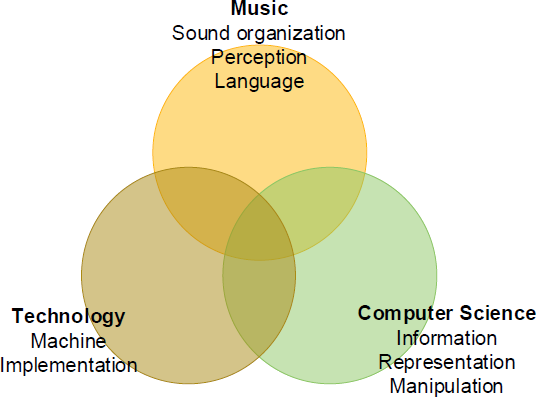
\includegraphics[width=0.6\linewidth]{00_Images/Res/02_chapter/01.png}
    \caption{Computer and music}
    \label{fig:computerandmusic}
\end{figure}

\subsection{Music}

Music can be defined in different ways:

\begin{itemize}
    \item Organized sound: Edgard Varèse defined music as "organized sound," where the organizer (musician, singer, composer, listener) plays a fundamental role.
    \item A category of perception: Music is deeply connected to human cognition.
    \item A language: Music is a form of communication that expresses moods, emotions, and thoughts.
\end{itemize}

\subsection{Computer Science}

A computer is a machine that manipulates data according to a list of instructions. The field of computing, as defined by the Association for Computing Machinery (ACM), is:

\begin{quote}
    "The systematic study of algorithmic processes that describe and transform information, including their theory, analysis, design, efficiency, implementation, and application."
\end{quote}

Computing involves:

\begin{itemize}
    \item Information representation
    \item Information manipulation
    \item Algorithmic processing
\end{itemize}

\subsection{Bringing Everything Together}

Computer music is the intersection of three key domains:

\begin{itemize}
    \item Music: Sound organization, perception, language.
    \item Computer Science: Information representation and manipulation.
    \item Technology: Machines and their implementation in creative processes.
\end{itemize}

This interdisciplinary approach forms the foundation of the course, preparing students to engage with music through computational and technological means.

\section{History of Computer Music}

\subsection{Early Mechanical and Electronic Instruments}

Before digital computers, various automatic instruments paved the way:

\begin{itemize}
    \item Ancient: Greek Aeolian Harp (2nd century BC), mechanical organs (1500s).
    \item 19th-20th Century: Electromechanical Piano (1867), Theremin (1920).
    \item 1950s: RCA Synthesizer (1959) and voltage-controlled synthesizers (1960s).
\end{itemize}

\subsection{The First Computer-Generated Music}

CSIRAC (1949) was the first computer to play music, programmed by Geoff Hill in Australia.

ILLIAC Suite (1957) by Lejaren Hiller and Leonard Isaacson was the first computer-composed piece.

\subsection{Major Developments in Computer Music}

\begin{itemize}
    \item 1957: Max Mathews developed Music I, the first digital sound synthesis program.
    \item 1976: IRCAM was founded in Paris, becoming a leading center for computer music research.
    \item 1983: The MIDI protocol standardized communication between digital instruments.
    \item 1986: Miller Puckette developed Max, the first graphical programming environment for music.
    \item 1989-1991: The rise of Digital Audio Workstations (Sound Tools, Cubase, Pro Tools) revolutionized music production.
\end{itemize}
